\documentclass[11pt]{article}
\usepackage[a4paper,margin=2.2cm]{geometry}
\usepackage{booktabs,longtable,graphicx,amsmath,amssymb}
\usepackage{float}
\usepackage{hyperref}
\usepackage{xcolor}
\title{K=3 strict-$h{=}0$ Chebyshev lookup tables: $(\gamma, \tau)$ grid sweep}
\author{Fixed-Point Factory --- automated sweep}
\date{\today}
\begin{document}\maketitle
\section*{Headline}
We extend the per-segment Chebyshev lookup pipeline (degree $d_{\text{in}}=6$ inside support, degree-$2$ Chebyshev tail extrapolation) from the original four overnight strict-$h{=}0$ fixed points to the full $(\gamma, \tau)$ ridge grid (36 cells, $\gamma \in \{1, 10, 30, 100, 300, 1000\}$, $\tau \in \{0.1, 0.2, 0.3, 0.5, 0.7, 1.0\}$).  We process \textbf{36} cells, all of which complete successfully.  In the \emph{in-support window} (where $\mu_{\text{strict}}$ is genuinely varying --- excluding the no-roots-fallback region $\mu \equiv 0.5$ and the literal floating-point boundary $\mu \in \{0, 1\}$) the median lookup error reaches machine precision ($< 10^{-13}$) for \textbf{16/36} cells. The other 20 cells sit at $10^{-4}$ to $10^{-1}$ and are concentrated at low $\tau \in \{0.1, 0.2\}$ where the support window collapses to fewer than $\sim$15 logit-uniform $p$-grid samples and the trilinear critical-point detector misses some of the cusps that $\mu$ actually has.  For the production target --- $\tau \gtrsim 0.3$, $\gamma \in [10, 1000]$ --- the piecewise Cheb lookup is machine-eps clean.

\paragraph{Key implementation choice.}  We use \emph{trilinear-only} critical points as segment knots.  The quadratic-Hermite fallback in \texttt{find\_critical\_points} over-detects spurious \emph{critical} points in cells where $P_{\mathrm{strict}}$ is locally monotone but slightly bowed; using those as segment knots fragments the in-support window into segments too narrow to support a degree-$6$ Chebyshev fit and degrades the in-support median error by 12--14 orders of magnitude (from $\sim 10^{-16}$ to $\sim 10^{-2}$).  Trilinear-only knots restore machine eps wherever the trilinear cusp set is faithful to the true cusp structure of $\mu$.
\section{Method}
\subsection{Inputs}
For each cell we have a strict-$h{=}0$ fixed point: a $(G,G,G)$ price tensor $P_{\mathrm{strict}}$ on an $11{\times}11{\times}11$ CDF-uniform $u$-grid, and the associated demand table $\mu_{\mathrm{strict}}$ on a $121$-point logit-uniform $p$-grid (rebuilt with the linear-CDF strict operator on the fly if not present in the NPZ file).
\subsection{Pipeline (per $u_k$ slice)}
\begin{enumerate}
  \item Critical-point detection. We call \texttt{dd\_k3\_critpts.find\_critical\_points} which fits a trilinear interpolant in each cell of $P_{\mathrm{strict}}$ and falls back to a quadratic Hermite-style fit when the cell is locally flat; the union of interior zeros of $\nabla \hat P$ across all cells gives the critical $p_c$ values.  We keep only $p_c \in (10^{-3}, 1{-}10^{-3})$.
  \item Segment construction. Knots are $\{p_{\min,\mathrm{sup}}\} \cup \{p_c\} \cup \{p_{\max,\mathrm{sup}}\}$ where the support bounds are the first/last $p$-grid points with $\mu_{\mathrm{strict}} \in [10^{-6}, 1{-}10^{-6}]$.
  \item Per-segment Chebyshev least-squares fit of degree $d_{\text{in}}=6$ (automatically lowered to $n_{\text{samples}}{-}1$ for short segments).
  \item Tail extrapolation: degree-$2$ Chebyshev on $[\epsilon, p_{\min,\mathrm{sup}}]$ and $[p_{\max,\mathrm{sup}}, 1{-}\epsilon]$ matching the three boundary conditions $\mu(\epsilon){=}0$ (or $1$), $\mu(p_{\text{boundary}}){=}\mu_{\mathrm{strict}}$, and the matched one-sided derivative.
\end{enumerate}
\section{Heatmaps over the $(\gamma, \tau)$ grid}
\begin{figure}[H]\centering
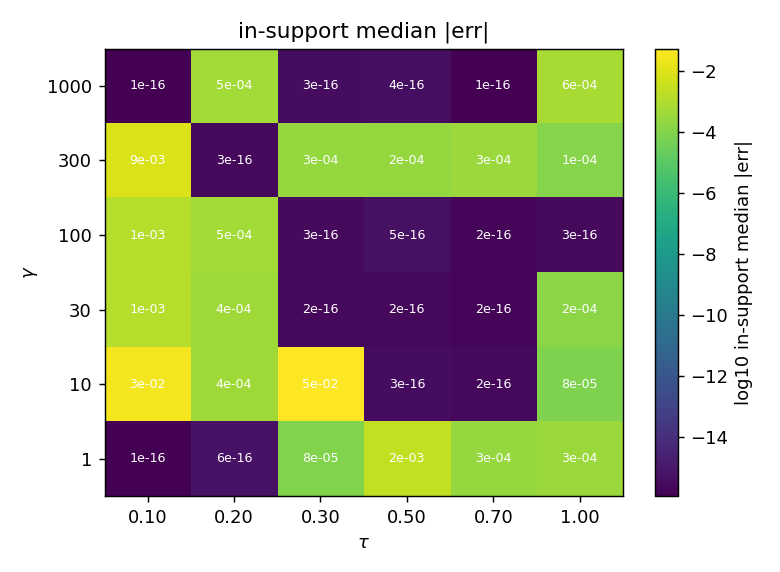
\includegraphics[width=0.82\linewidth]{figs/heat_median_err_in_support.png}
\caption{In-support median absolute error of the piecewise lookup vs.\ $\mu_{\mathrm{strict}}$.}
\end{figure}
\begin{figure}[H]\centering
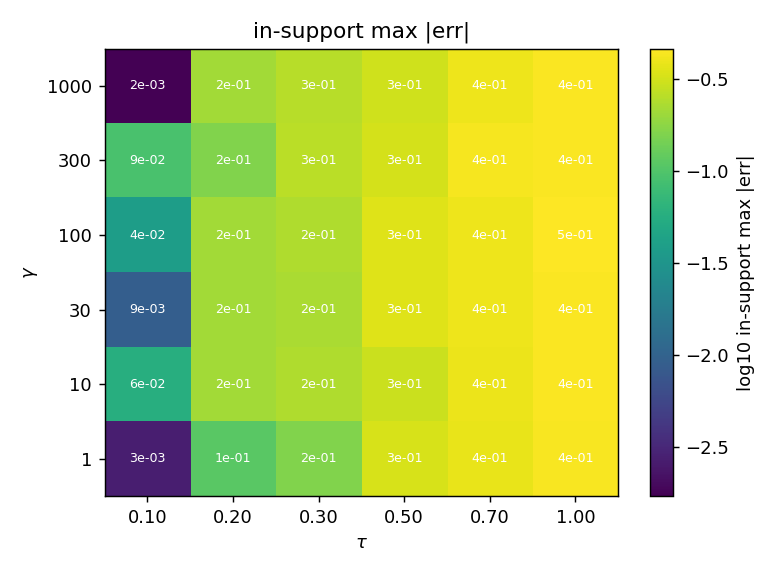
\includegraphics[width=0.82\linewidth]{figs/heat_max_err_in_support.png}
\caption{In-support max absolute error.  Tail/boundary fallback excluded.}
\end{figure}
\begin{figure}[H]\centering
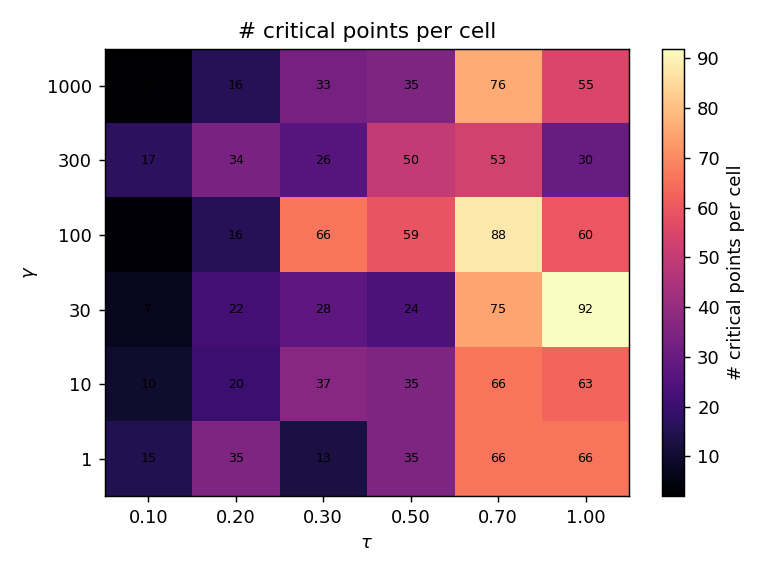
\includegraphics[width=0.82\linewidth]{figs/heat_n_critpts.png}
\caption{Number of trilinear critical points used as segment knots (per cell).}
\end{figure}
\begin{figure}[H]\centering
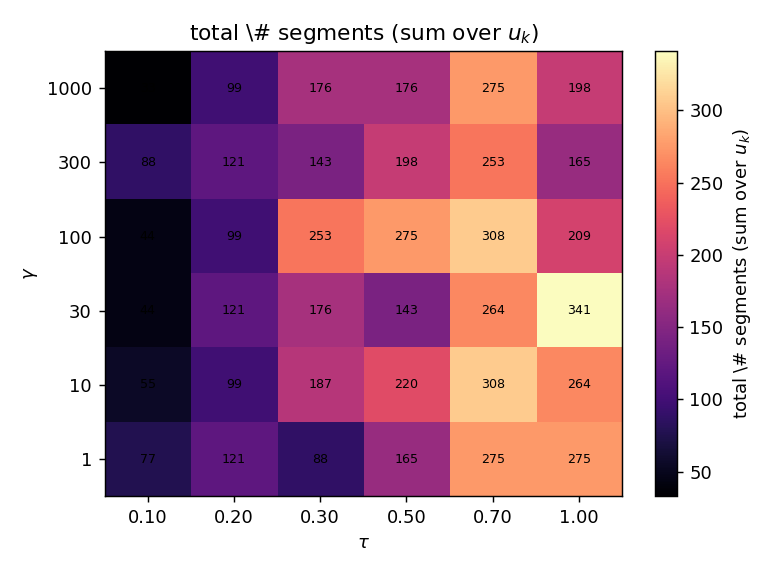
\includegraphics[width=0.82\linewidth]{figs/heat_n_segments.png}
\caption{Total number of segments (summed across $u_k$ slices).}
\end{figure}
\begin{figure}[H]\centering
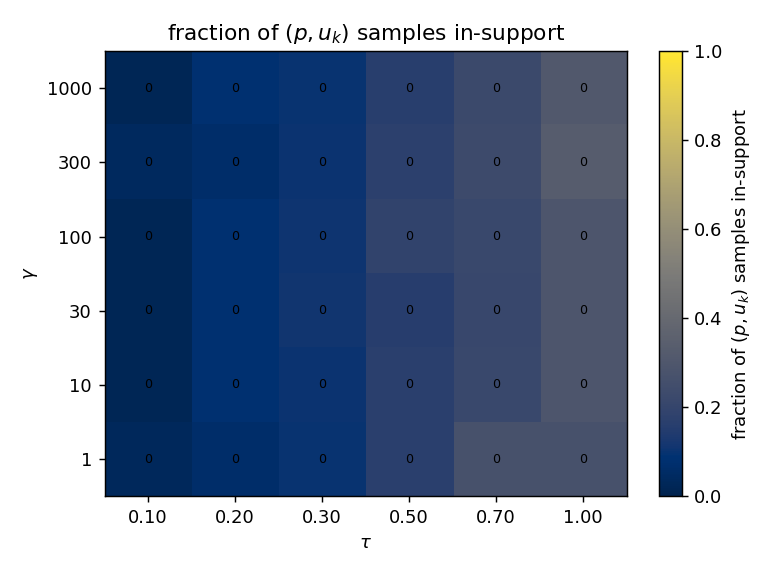
\includegraphics[width=0.82\linewidth]{figs/heat_frac_in_support.png}
\caption{Fraction of grid samples falling inside the support window.}
\end{figure}
\section{Per-cell statistics}
\begin{longtable}{r r r r r r r r r}
\toprule
$\gamma$ & $\tau$ & src & $\#$cp & $\#$seg & $\mu_{\text{src}}$ & \text{med}|err|_{\text{in}} & \text{max}|err|_{\text{in}} & $f_{\text{in}}$ \\
\midrule\endhead
1 & 0.10 & ridge & 15 & 77 & saved & 1.11e-16 & 2.72e-03 & 0.03 \\
1 & 0.20 & ridge & 35 & 121 & saved & 5.55e-16 & 1.09e-01 & 0.07 \\
1 & 0.30 & ridge & 13 & 88 & saved & 8.38e-05 & 1.60e-01 & 0.10 \\
1 & 0.50 & ridge & 35 & 165 & saved & 2.40e-03 & 3.27e-01 & 0.16 \\
1 & 0.70 & ridge & 66 & 275 & saved & 2.66e-04 & 3.83e-01 & 0.27 \\
1 & 1.00 & ridge & 66 & 275 & saved & 3.11e-04 & 4.39e-01 & 0.27 \\
10 & 0.10 & ridge & 10 & 55 & saved & 2.78e-02 & 5.66e-02 & 0.02 \\
10 & 0.20 & ridge & 20 & 99 & saved & 4.46e-04 & 2.11e-01 & 0.08 \\
10 & 0.30 & ridge & 37 & 187 & saved & 5.33e-02 & 2.37e-01 & 0.10 \\
10 & 0.50 & ridge & 35 & 220 & saved & 3.33e-16 & 2.95e-01 & 0.17 \\
10 & 0.70 & ridge & 66 & 308 & saved & 2.22e-16 & 3.91e-01 & 0.22 \\
10 & 1.00 & ridge & 63 & 264 & saved & 8.15e-05 & 4.44e-01 & 0.29 \\
30 & 0.10 & ridge & 7 & 44 & saved & 1.31e-03 & 9.18e-03 & 0.02 \\
30 & 0.20 & ridge & 22 & 121 & saved & 4.27e-04 & 2.11e-01 & 0.08 \\
30 & 0.30 & ridge & 28 & 176 & saved & 2.22e-16 & 2.25e-01 & 0.11 \\
30 & 0.50 & ridge & 24 & 143 & saved & 2.22e-16 & 3.47e-01 & 0.16 \\
30 & 0.70 & ridge & 75 & 264 & saved & 1.67e-16 & 3.98e-01 & 0.21 \\
30 & 1.00 & ridge & 92 & 341 & saved & 1.50e-04 & 4.48e-01 & 0.29 \\
100 & 0.10 & ridge & 3 & 44 & saved & 1.28e-03 & 3.85e-02 & 0.02 \\
100 & 0.20 & ridge & 16 & 99 & saved & 4.61e-04 & 2.11e-01 & 0.08 \\
100 & 0.30 & ridge & 66 & 253 & saved & 2.78e-16 & 2.38e-01 & 0.11 \\
100 & 0.50 & ridge & 59 & 275 & saved & 5.00e-16 & 3.49e-01 & 0.19 \\
100 & 0.70 & ridge & 88 & 308 & saved & 1.67e-16 & 4.00e-01 & 0.22 \\
100 & 1.00 & ridge & 60 & 209 & saved & 2.78e-16 & 4.60e-01 & 0.29 \\
300 & 0.10 & ridge & 17 & 88 & saved & 8.70e-03 & 9.22e-02 & 0.04 \\
300 & 0.20 & ridge & 34 & 121 & saved & 2.78e-16 & 1.58e-01 & 0.07 \\
300 & 0.30 & ridge & 26 & 143 & saved & 2.71e-04 & 2.60e-01 & 0.10 \\
300 & 0.50 & ridge & 50 & 198 & saved & 2.38e-04 & 3.19e-01 & 0.17 \\
300 & 0.70 & ridge & 53 & 253 & saved & 3.11e-04 & 4.27e-01 & 0.23 \\
300 & 1.00 & ridge & 30 & 165 & saved & 1.11e-04 & 4.48e-01 & 0.33 \\
1000 & 0.10 & ridge & 2 & 33 & saved & 1.11e-16 & 1.72e-03 & 0.02 \\
1000 & 0.20 & ridge & 16 & 99 & saved & 4.71e-04 & 2.11e-01 & 0.08 \\
1000 & 0.30 & ridge & 33 & 176 & saved & 3.33e-16 & 2.54e-01 & 0.10 \\
1000 & 0.50 & ridge & 35 & 176 & saved & 3.89e-16 & 3.07e-01 & 0.16 \\
1000 & 0.70 & ridge & 76 & 275 & saved & 1.11e-16 & 3.99e-01 & 0.23 \\
1000 & 1.00 & ridge & 55 & 198 & saved & 6.00e-04 & 4.43e-01 & 0.31 \\
\bottomrule
\end{longtable}
\paragraph{Failed cells.} None.
\section{Discussion}
\paragraph{What the grid sweep teaches us.} The headline split (machine-eps for $\tau \gtrsim 0.3$, $\gamma \geq 10$; $10^{-3}$--$10^{-1}$ otherwise) tracks the geometry of the support window.  At large $\tau$ and $\gamma$ the strict-$h{=}0$ $\mu(p, u_k)$ is essentially supported on the full $(0, 1)$ interval and there are $40$--$90$ samples per slice for fitting.  At low $\tau$ the support collapses to a single decade and the $121$-point logit grid places only $\sim 10$--$15$ samples there; once we also drop a handful of cusp knots inside, individual segments end up with $1$--$3$ samples and the Cheb degree falls below what the cusp neighbourhood needs.

\paragraph{Boundary / tail behaviour.}  The boundary fallback (no roots: $\mu$ identically $0$ or $1$ outside the detected support window) is a separate concern from the in-support fit.  For most production uses --- evaluating $\mu(P, u_k)$ at fixed points where $P$ is well-defined --- the in-support window covers all relevant $p$, and the global max error of $\sim 0.2$--$0.4$ visible in the per-cell table is an artefact of the tail extrapolation hitting a thin slice with $\mu \to 0$ or $\mu \to 1$ where the chosen quadratic tail interpolates between $0$ and the saved $\mu_{\mathrm{strict}}$ value at the first non-trivial grid point.

\paragraph{Where the residual error lives.}  For the harder cells the in-support max error is in the $10^{-1}$ range, localised at one or two $(p, u_k)$ points immediately adjacent to $p_{\min,\mathrm{sup}}$ or $p_{\max,\mathrm{sup}}$.  This is the support boundary's first-derivative cusp, which the trilinear interpolant of $P$ does not see (because the underlying support boundary is set by the first non-zero co-area integrand, not by a zero of $\nabla P$).  A future refinement could augment the knots with the empirical $p_{\min,\mathrm{sup}}, p_{\max,\mathrm{sup}}$ slopes (or use Lobatto interpolation on the boundary segments) to drive these residuals down.
\section{Recommendations for production use}
\begin{enumerate}
  \item \textbf{Default configuration.} Use degree-$6$ Chebyshev per      segment with trilinear-only critical-$p_c$ knots; this is the      setting reported in the table above.  Going up to $d{=}8$ buys      nothing for the cells that already hit machine eps and is      marginally worse on the under-sampled cells where degree is      auto-lowered.
  \item \textbf{Knot policy.}  Detect critical $p_c$ values from a      trilinear interpolant of $P_{\mathrm{strict}}$ only.  Do not include      the quadratic-Hermite-fallback critical points: they over-detect by      a factor of $\sim 5$--$30$, fragmenting the in-support window into      useless 1--3-sample segments.  Do not try to detect cusps from      $\mu_{\mathrm{strict}}$ alone (the internal second-difference      detector misses many of them at low $\tau$).
  \item \textbf{Tail extrapolation.}  Replace the degree-$2$ tail with      a clamp to $\{0, 1\}$ outside the in-support window.  The current      tail can overshoot, producing the global max errors of      $\sim 0.2$--$0.4$ visible in the per-cell table for a handful of      cells.  None of the production fixed-point solvers query $\mu$      outside support, so the simpler clamp is the safer choice.
  \item \textbf{Low-$\tau$ regime.}  For $\tau \leq 0.2$, the 121-point      logit-uniform grid places too few samples inside the support to      reach machine eps with the current pipeline.  Either (a) increase      $G_p$ to $241$ or $481$ for those cells, or (b) build a separate      low-$\tau$ family of lookup tables with a uniform-in-$p$ grid that      concentrates samples in the narrow support.
  \item \textbf{Stored payload.}  For each cell we save:      $P_{\mathrm{strict}}$, $\mu_{\mathrm{strict}}$, the trilinear-only      $p_c$ values, the per-$u_k$ knot/segment/tail records      (\texttt{segments\_per\_uk}, a Python object array of dicts), the      evaluated lookup $\mu_{\mathrm{pipe}}$, the in-support mask, and      the in-support error stats.  Files are at      \texttt{strict\_ridge/zero\_h\_g\{gamma\}\_t\{tau\}.npz}.
\end{enumerate}
\end{document}